\chapter{恒定电流}

\section{电流 电阻 电功及电功率}





1.电流

(1)形成的条件:导体中有\_\_自由电荷\_\_;导体两端存在\_\_电压\_\_.

(2)标矢性:电流是标量,\_\_正电荷\_\_定向移动的方向规定为电流的方向.

(3)两个表达式:\ding{172}定义式$I=\dfrac{q}{t}$;\ding{173}决定式$I=\dfrac{U}{R}$.

2.电阻、电阻定律

(1)电阻:反映了\_\_导体对电流阻碍作用\_\_的大小,表达式为$R=\dfrac{U}{I}$.

(2)电阻定律:同种材料的导体,其电阻跟它的\_\_长度\_\_成正比,与它的\_\_横截面积\_\_成反比,导体的电阻还与构成它的材料有关.表达式为$R=\rho \dfrac{L}{S}$.

(3)电阻率:

\ding{172}物理意义:反映导体的\_\_导电性能\_\_,是导体材料本身的属性;

\ding{173}电阻率与温度的关系:金属的电阻率随温度升高而\_\_增大\_\_;半导体的电阻率随温度升高而\_\_减小\_\_.

3.部分电路欧姆定律及其应用

(1)内容:导体中的电流跟导体两端的\_\_电压\_\_成正比,跟导体的\_\_电阻\_\_成反比.

(2)表达式:$I=\dfrac{U}{R}$.

(3)适用范围:金属导电和电解液导电,不适用于气体导电或半导体元件.

(4)导体的伏安特性曲线(I-U)图线

\begin{center}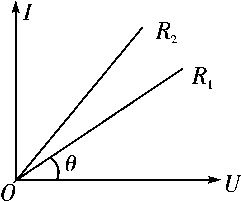
\includegraphics[width=1.09444in,height=0.91528in]{media/image307.png}\end{center}

\ding{172}比较电阻的大小:图线的斜率$k=\tan \theta=\dfrac{I}{U}=\dfrac{1}{R}$,图中$R_1$\textgreater$R_2$(选填``\textgreater''\,``\textless''或``='');

\ding{173}线性元件:伏安特性曲线是过原点的直线的电学元件,适用于欧姆定律;

\ding{174}非线性元件:伏安特性曲线不是过原点的直线的电学元件,不适用于欧姆定律.

4.电功率、焦耳定律

(1)电功:电路中\_\_电场力\_\_移动电荷做的功.表达式为$W=q U=U I t$.

(2)电功率:单位时间内电流做的功.表示电流做功的\_\_快慢\_\_.表达式为$P=\dfrac{W}{t}=UI$.

\ding{172}纯电阻用电器:电功率$P=I U=I^{2} R=\dfrac{U^{2}}{R}$.

\ding{173}非纯电阻用电器:电功率只能是$P=UI$.

(3)焦耳定律:电流通过导体产生的\_\_热量\_\_跟电流的二次方成正比,跟导体的电阻及通电时间成正比.表达式为$Q=I^2Rt$.

\ding{172}纯电阻用电器:电热$Q=I Ut=I^{2} Rt=\dfrac{U^{2}}{R}t$.

\ding{173}非纯电阻用电器:电热只能是$Q=I^2Rt$.


\newpage
\subsection{对电流表达式的理解}


\begin{longtable}[]{@{}m{1.5cm}m{4cm}m{6cm}@{}}
\toprule
& 公式及适用范围 & 字母含义\tabularnewline
\midrule
\endhead

定义式
& \begin{minipage}[t]{0.30\columnwidth}\raggedright
$I=\dfrac{q}{t}$

一切电路\strut
\end{minipage} & \begin{minipage}[t]{0.50\columnwidth}\raggedright
q为时间t内通过导体横截面的电荷量\strut
\end{minipage}\tabularnewline
\begin{minipage}[t]{0.30\columnwidth}\raggedright
微观式\strut
\end{minipage} & \begin{minipage}[t]{0.30\columnwidth}\raggedright
$I=nqSv$

一切电路\strut
\end{minipage} & \begin{minipage}[t]{0.50\columnwidth}\raggedright
n:导体单位体积内的自由电荷数

q:每个自由电荷的电荷量

S:导体横截面积

v:电荷定向移动速率\strut
\end{minipage}\tabularnewline
\begin{minipage}[t]{0.30\columnwidth}\raggedright
决定式\strut
\end{minipage} & \begin{minipage}[t]{0.30\columnwidth}\raggedright
$I=\dfrac{U}{R}$

金属、电解液\strut
\end{minipage} & \begin{minipage}[t]{0.50\columnwidth}\raggedright
U:导体两端的电压

R:导体本身的电阻\strut
\end{minipage}\tabularnewline
\bottomrule
\end{longtable}

\begin{center}
\includegraphics[width=0.70764in,height=0.12292in]{media/image37.png}\end{center}
\begin{center}
	\textbf{电流微观表达式的相关说明}
\end{center}

(1)判断某个量与其他量的变化关系,可以根据公式推导出该物理量的表达式,就能看出该物理量与其他量是否有关,以及随其他量的变化规律.

(2)电流的微观表达式在金属导体、静电除尘、电视机显像管等问题中都有应用.

\subsection{电阻定律的理解及应用}

两个公式的对比

\begin{longtable}[]{@{}m{1.2cm}m{6cm}m{6cm}@{}}
\toprule
公式 & $R=\rho \dfrac{L}{S}$ & $I=\dfrac{U}{R}$\tabularnewline
\midrule
\endhead
\multirow{3}{1cm}{区别} & 电阻的决定式 & 电阻的定义式\tabularnewline
& 说明了电阻的决定因素 &
提供了一种测定电阻的方法,并不说明电阻与U和I有关\tabularnewline
& 只适用于粗细均匀的金属导体和浓度均匀的电解液 &
适用于任何纯电阻导体\tabularnewline
相同点 &\multicolumn{2}{l}{ 都不能反映电阻的实质(要用微观理论解释) }\tabularnewline
\bottomrule
\end{longtable}

\begin{center}
\includegraphics[width=0.70764in,height=0.12292in]{media/image37.png}\end{center}
\begin{center}
	\textbf{导体形变后电阻的分析方法}
\end{center}

某一导体的形状改变后,讨论其电阻变化应抓住以下三点:

(1)导体的电阻率不变,因其由导体材料本身决定.

(2)导体的体积不变,由V=lS可知l与S成反比.

(3)在$\rho$、l、S都确定之后,应用电阻定律$R=\rho \dfrac{L}{S}$求解.
\newpage
\subsection{欧姆定律与伏安特性曲线的理解及应用}


1.图线的意义

(1)由于导体的导电性能不同,所以不同的导体有不同的伏安特性曲线.

(2)伏安特性曲线上每一点的电压坐标与电流坐标的比值,对应这一状态下的电阻.

2.图线的区别

(1)图甲中图线a、b表示线性元件,图乙中图线c、d表示非线性元件.

(2)在伏安特性曲线中,线性元件图线的斜率表示电阻的倒数,斜率越大,电阻越小,故$R_a$\textless $R_b$(如图甲所示).

(3)图线c的斜率增大,电阻减小;图线d的斜率减小,电阻增大(如图乙所示).

\begin{center}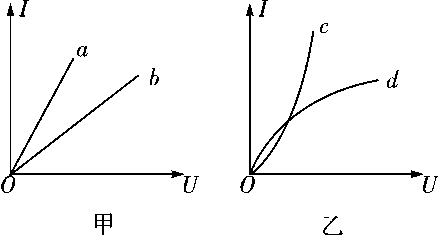
\includegraphics[width=1.99028in,height=1.06597in]{media/image311.png}\end{center}

(4)c、d图线上某点切线的斜率不是电阻的倒数.

{[}例3{]}(2017·四川成都诊断)小灯泡通电后其电流I随所加电压U变化的图线如图所示,P为图线上一点,PN为图线在P点的切线,PQ为U轴的垂线,PM为I轴的垂线,则下列说法中正确的是( D )

\begin{center}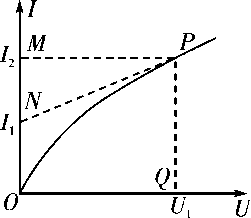
\includegraphics[width=1.14167in,height=0.99028in]{media/image312.png}\end{center}

A.随着所加电压的增大,小灯泡的电阻减小

B.对应P点,小灯泡的电阻为$R=\dfrac{U_{1}}{I_{1}}$

C.对应P点,小灯泡的电阻为$R=\dfrac{U_{1}}{I_{2}-I_{1}}$

D.对应P点,小灯泡的功率为图中矩形PQOM所围面积

\begin{center}
\includegraphics[width=0.70764in,height=0.12292in]{media/image34.png}\end{center}
\begin{center}
	\textbf{运用伏安特性曲线求电阻应注意的问题}
\end{center}

(1)如图所示.非线性元件的I-U图线是曲线,导体电阻$R_{N}=\dfrac{U_{N}}{I_{N}}$,即电阻等于图线上点$\left(U_{N}, I_{N}\right)$与坐标原点连线的斜率的倒数,而不等于该点切线斜率的倒数,即$R \neq \dfrac{\Delta U}{\Delta I}$.

(2)I-U图线中的斜率$k=\dfrac{1}{R}$,斜率k不能理解为$k=\tan \alpha$($\alpha$为图线与U轴的夹角),因坐标轴的单位可根据需要人为规定,同一电阻在坐标轴单位不同时倾角$\alpha$是不同的.

\begin{center}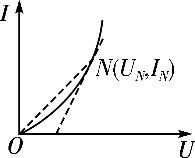
\includegraphics[width=0.88681in,height=0.71667in]{media/image313.png}\end{center}

\subsection{电功和电热 电功率和热功率}
纯电阻电路与非纯电阻电路的比较

用电器纯电阻$W=Q W=U I t=P^{2} R t=\dfrac{U^{2}}{R} t P=U I=P^{2} R=\dfrac{U^{2}}{R}$如电阻、电炉、白炽灯等非纯电阻$W>Q W=U I t=P^{2} R t=\dfrac{U^{2}}{R} t P=U I=P^{2} R=\dfrac{U^{2}}{R}$其他如电风扇、电动机、电解槽等

{[}例4{]}如图所示是一提升重物用的直流电动机工作时的电路图.电动机内电阻r=0.8
$\Omega$,电路中另一电阻R=10 $\Omega$,直流电压U=160 V,电压表示数UV=110 V.试求:

\begin{center}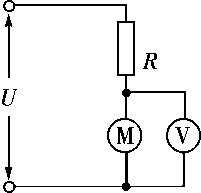
\includegraphics[width=0.91528in,height=0.87708in]{media/image314.png}\end{center}

(1)通过电动机的电流;

(2)输入电动机的电功率;

(3)若电动机以v=1 m/s匀速竖直向上提升重物,求该物的质量.(g取10 $m/s^2$)
\begin{solution}
	(1)5 A (2)550 W (3)53 kg
	
	(1)由电路中的电压关系可得电阻R的分压$U_{R}=U-U_{\mathrm{V}}=(160-110) \mathrm{V}=50 \mathrm{V}$,流过电阻R的电流$I_{R}=\dfrac{U_{R}}{R}=\dfrac{50}{10} \mathrm{A}=5A$,即通过电动机的电流$I_{\mathrm{M}}=I_{R}=5 \mathrm{A}$.

(2)电动机的分压$U_{\mathrm{M}}=U_{\mathrm{V}}=110 \mathrm{V}$,输入电动机的功率$P_{\text {电 }}=I_{\mathrm{M}} U_{\mathrm{M}}=550 \mathrm{W}$.

(3)电动机的发热功率$P_{\text {热 }}=I_{\mathrm{M}}^2 r=20 \mathrm{W}$,电动机输出的机械功率$P_{\text {出 }}=P_{\text {电 }}-P_{\text {热 }}=530 \mathrm{W}, \quad$ 又因 $P_{\text {出 }}=m g v,$ 所以 $m=\dfrac{P_{\text {出 }}}{g v}=53 kg$.
\end{solution}


\begin{center}
\includegraphics[width=0.70764in,height=0.12292in]{media/image34.png}\end{center}
\begin{center}
	\textbf{非纯电阻问题的``四大注意''}
\end{center}



(1)无论是纯电阻还是非纯电阻,电功均为$W=UIt$,电热均为$Q=I^2Rt$.

(2)处理非纯电阻的计算问题时,要善于从能量转化的角度出发,紧紧围绕能量守恒,利用``电功=电热+其他能量''寻找等量关系求解.

(3)非纯电阻在一定条件下可当作纯电阻处理,如电动机卡住不转时即为纯电阻.

(4)若电路中,为电动机与纯电阻串联.在求电动机电压和电流时,不能对电动机应用欧姆定律,应对其他纯电阻元件分析,间接得到电动机电压和电流.

\newpage
\section{电路 闭合电路的欧姆定律}

1.串、并联电路的特点

(1)特点对比

\begin{longtable}[]{@{}m{1cm}m{6cm}m{6cm}@{}}
\toprule
& 串联 & 并联\tabularnewline
\midrule
\endhead
电流 & $I=I_{1}=I_{2}=\ldots=I_{n}$ &
$I=I_{1}+I_{2}+\ldots+I_{n}$\tabularnewline
电压 & $U=\quad U_{1}+U_{2}+\ldots+U_{n}$ &
$U=U_{1}=U_{2}=\ldots=U_{n}$\tabularnewline
电阻 & $R=R_{1}+R_{2}+\ldots+R_{n}$ &
$\dfrac{1}{R}=\dfrac{1}{R_{1}}+\dfrac{1}{R_{2}}+\ldots+\dfrac{1}{R_{n}}$\tabularnewline
\bottomrule
\end{longtable}

(2)几个常用的推论

\ding{172}串联电路的总电阻\_\_大于\_\_其中任一部分电路的总电阻.

\ding{173}并联电路的总电阻\_\_小于\_\_其中任一支路的总电阻,且小于其中最小的电阻.

\ding{174}无论电阻怎样连接,每一段电路的总的消耗电功率P总是等于各个电阻消耗电功率之和.

\ding{175}无论电路是串联还是并联,电路中任意一个电阻变大时,电路的总电阻变大.

2.电源的电动势和内阻

(1)电动势

\ding{172}电动势的计算:非静电力搬运电荷所做的功与搬运的电荷量的比值,$E=\dfrac{W}{q}$;

\ding{173}电动势的物理含义:电动势表示电源\_\_把其他形式的能转化成电势能\_\_本领的大小,在数值上等于电源没有接入电路时两极间的电压.

(2)内阻:电源内部导体的电阻.

3.闭合电路的欧姆定律

(1)闭合电路欧姆定律

\ding{172}内容:闭合电路里的电流跟电源的电动势成\_\_正比\_\_,跟内、外电阻之和成\_\_反比\_\_;

\ding{173}公式:$I=\dfrac{E}{R+r}$(只适用于纯电阻电路);

\ding{174}其他表达形式

a.电势降落表达式:$E=U_{\text{外}}$+$U_{\text {内 }} $或$E=U_{\text{外}}$  $+I r$;

b.能量表达式:$E I=U I+I^{2} r$.

(2)路端电压与外电阻的关系

\ding{172}一般情况:$U=I R=\dfrac{E}{R+r} R=\dfrac{E}{1+\dfrac{r}{R}}$,当R增大时,U\_\_增大\_\_;

\ding{173}特殊情况:

a.当外电路断路时,I=0,U=\_\_E\_\_;

b.当外电路短路时,$I_{\text {短 }}=\dfrac{E}{r}$,U=0.

\newpage
\subsection{闭合电路的功率及效率问题}

\begin{longtable}[]{@{}m{4cm}m{10cm}@{}}
\toprule
\multirow{2}{3cm}{电源总功率} & 任意电路 $P_{\text {总 }}=E I=P_{\text {出十 }} P$\tabularnewline

& 纯电阻电路 $P_{\text {总 }}=I^{2}(R+r)=\dfrac{E^{2}}{R+r}$\tabularnewline
电源内部消耗的功率 & $P_{\text {内 }}=P^{2} r=P_{\text {总 }}-P_{\text {出 }}$\tabularnewline
\multirow{2}{3cm}{电源的输出功率} & 任意电路 $P_{\text {出 }}=U I=P_{\text {总 }}-P$\tabularnewline
& 纯电阻电路 $P_{\text {出 }}=P^{2} R=\dfrac{E^{2} R}{(R+r)^{2}}$\tabularnewline
$P_{\text{出}}$外电阻R的关系 &
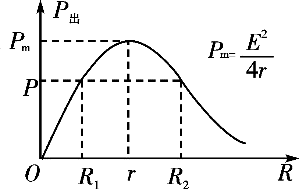
\includegraphics[width=1.35833in,height=0.85833in]{media/image320.png}\tabularnewline
\multirow{2}{3cm}{电源的效率} & $\eta=\dfrac{P_{\text {出 }}}{P_{\text {总 }}} \times 100 \%=\dfrac{U}{E} \times 100 \%$\tabularnewline
& 纯电阻电路 $\eta=\dfrac{R}{R+r} \times 100 \%$\tabularnewline
\bottomrule
\end{longtable}

由P出与外电阻R的关系图象可知

\ding{172}当R=r时,电源的输出功率最大为$P_{\mathrm{m}}=\dfrac{E^{2}}{4 r}$;

\ding{173}当R\textgreater r时,随着R的增大输出功率越来越小;

\ding{174}当R\textless r时,随着R的增大输出功率越来越大;

\ding{175}当$P_{\text {出 }}<P_{\mathrm{m}}$时,每个输出功率对应两个外电阻$R_1$和$R_2$,且$R_1$$R_2$=$r_2$.

\begin{center}
\includegraphics[width=0.70764in,height=0.12292in]{media/image13.png}\end{center}
\begin{center}
	\textbf{闭合电路欧姆定律中功率的最值问题}
\end{center}

(1)定值电阻的功率$P_{\text {定 }}=I^{2} R$

R为定值电阻,$P_{\text {定 }}$只与电流有关系,当$R_{\text {外 }}$最大时,I最小$P_{\text {定 }}$最小,当$R_{\text {外 }}$最小时,I最大$P_{\text {定 }}$最大.

(2)电源的输出功率$P_{\text {出 }}=\dfrac{E^{2} R_{\text {外 }}}{\left(r+R_{\text {外 }}\right)^{2}}=\dfrac{E^{2}}{\dfrac{\left(R_{\text {外 }}-r\right)^{2}}{R_{\text {外 }}}+4 r}$

当$R_{\text {外 }}=r$时,P出功率最大.

(3)变化电阻的功率的最大值

利用等效思想,把除变化电阻之外的其他的定值电阻等效成电源的内阻$r^{\prime}$,则变化电阻的功率即为等效以后的电源的输出功率,即当R变$R$ 变 $=r^{\prime}$时,$P_{\text {变 }}$有最大值.

\newpage
\subsection{电路的动态分析}

1.动态分析特点

断开或闭合开关、滑动变阻器的滑片移动、电阻增大或减小导致电路电压、电流、功率等的变化.

2.电路动态分析的方法

(1)程序法

电路结构的变化$\rightarrow$R的变化$\rightarrow$$R_{\text {总 }}$的变化$\rightarrow$$I_{\text {总 }}$的变化$\rightarrow$U端的变化$\rightarrow$固定支路的变化$\rightarrow$变化支路I、U、P的变化.

(2)``串反并同''结论法

\ding{172}所谓``串反'',即某一电阻增大时,与它串联或间接串联的电阻中的电流、两端电压、电功率都将减小,反之则增大.

\ding{173}所谓``并同'',即某一电阻增大时,与它并联或间接并联的电阻中的电流、两端电压、电功率都将增大,反之则减小.

即:$\left.\begin{array}{l}U_{\text {串 }} \downarrow \\ I_{\text {串 }} \downarrow \\ P_{\text {串 }}\downarrow\end{array}\right\} \leftarrow R \uparrow \rightarrow\left\{\begin{array}{l}U_{\text {并 }} \uparrow \\ I_ \text { 并 } \uparrow \\ P_\text { 并 }{\uparrow}\end{array}\right.$

(3)极限法

对于因滑动变阻器的滑片滑动引起电路变化的问题,可将滑动变阻器的滑片分别滑至两个极端去讨论.此时要注意是否出现极值情况,即变化是否是单调变化.

(4)特殊值法

对于某些电路问题,可以代入特殊值进行判定,从而得出结论.

{[}例2{]}(2018·东北育才模拟)如图所示电路中,电源电动势为E,电源内阻为r,串联的固定电阻为$R_2$,滑动变阻器的总电阻为$R_1$,电阻大小关系为$R_1$=$R_2$=r,则在滑动触头P从a端移动到b端的过程中,下列描述中正确的是( B )

\begin{center}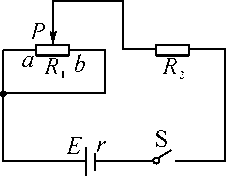
\includegraphics[width=1.02847in,height=0.80208in]{media/image322.png}\end{center}

A.电路中的总电流先增大后减小

B.电路的路端电压先增大后减小

C.电源的输出功率先增大后减小

D.滑动变阻器$R_1$上消耗的功率先减小后增大

\begin{center}
\includegraphics[width=0.70764in,height=0.12292in]{media/image25.png}\end{center}
\begin{center}
	\textbf{电路动态分析思路}
\end{center}

\begin{center}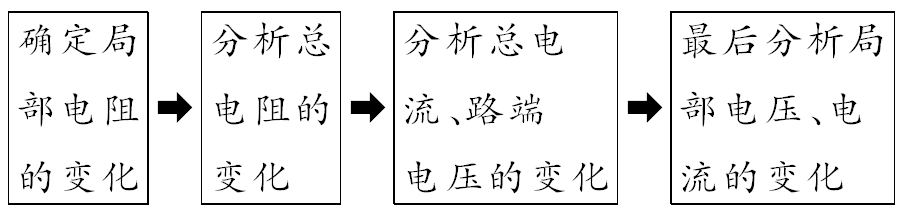
\includegraphics[width=2.81111in,height=0.67014in]{media/image323.png}\end{center}

\newpage
\subsection{含电容器电路的分析}

1.电容器的简化处理:简化电路时可以把电容器所处电路作为断路,简化电路时可以去掉,求电荷量时在相应位置再补上.

2.电阻的简化处理:电路稳定后,与电容器同支路的电阻是一个等势体,相当于导线.

3.电荷变化量的计算:电路中电流、电压的变化可能会引起电容器的充、放电.若电容器两端电压升高,电容器将充电,若电压降低,电容器将通过与它连接的电路放电.可由$\Delta Q=C \Delta U$计算电容器上电荷量的变化.

\subsection{两种U-I图线的比较及应用}

\begin{longtable}[]{@{}m{2.5cm}m{5cm}m{5cm}@{}}
\toprule
& 电源U-I图象 & 电阻U-I图象\tabularnewline
\midrule
\endhead
图形 &
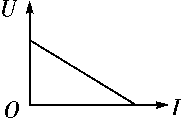
\includegraphics[width=0.82083in,height=0.5375in]{media/image325.png} &
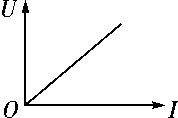
\includegraphics[width=0.81111in,height=0.5375in]{media/image326.png}\tabularnewline
物理意义 & 路端电压随电流的变化规律 &
电阻两端电压随电流的变化规律\tabularnewline
截距 & 与纵轴交点表示电源电动势E,与横轴交点表示短路电流$\dfrac{E}{r}$ &
过坐标轴原点,表示没有电压时电流为零\tabularnewline
坐标的乘积UI & 表示电源的输出功率 & 表示电阻消耗的功率\tabularnewline
坐标的U、I比值 & 表示外电阻的大小,不同点对应的外电阻大小不同 &
每一点对应的比值均等大,表示此电阻的大小不变\tabularnewline
斜率的绝对值 & 内电阻r & 电阻大小\tabularnewline
\bottomrule
\end{longtable}



\begin{center}
\includegraphics[width=0.70764in,height=0.12292in]{media/image13.png}\end{center}
\begin{center}
	\textbf{分析U-I图象的一般思路}
\end{center}


(1)明确纵、横坐标的物理意义.

(2)明确图象的截距、斜率及交点的意义.

(3)找出图线上对应状态的参量或关系式.

(4)结合相关概念或规律进行分析、计算


\subsection{电路故障的分析与判断}

1.故障特点

\ding{172}断路特点:表现为路端电压不为零而电流为零;

\ding{173}短路特点:用电器或电阻发生短路,表现为有电流通过电路但用电器或电阻两端电压为零.

2.检查方法

\ding{172}电压表检测:如果电压表示数为零,则说明可能在并联路段之外有断路,或并联路段短路;

\ding{173}电流表检测:当电路中接有电源时,可用电流表测量各部分电路上的电流,通过对电流值的分析,可以确定故障的位置.在运用电流表检测时,一定要注意电流表的极性和量程;

\ding{174}欧姆表检测:当测量值很大时,表示该处断路,当测量值很小或为零时,表示该处短路.在运用欧姆表检测时,电路一定要切断电源;

\ding{175}假设法:将整个电路划分为若干部分,然后逐一假设某部分电路发生某种故障,运用闭合电路或部分电路的欧姆定律进行推理.


